\documentclass[a4paper,12pt]{article}

\usepackage[utf8]{inputenc}
\usepackage{lmodern}
\usepackage[margin=1cm]{geometry}
\usepackage{amsmath}
\usepackage{graphicx}
\usepackage{xcolor}
\usepackage{caption}
\usepackage{tikz}
\usetikzlibrary{arrows.meta,positioning,shapes.geometric,calc,fit}

\pagestyle{empty}

\begin{document}
\begin{figure}[p]
  \centering
  \makebox[\textwidth][c]{\resizebox{1.08\textwidth}{!}{%
  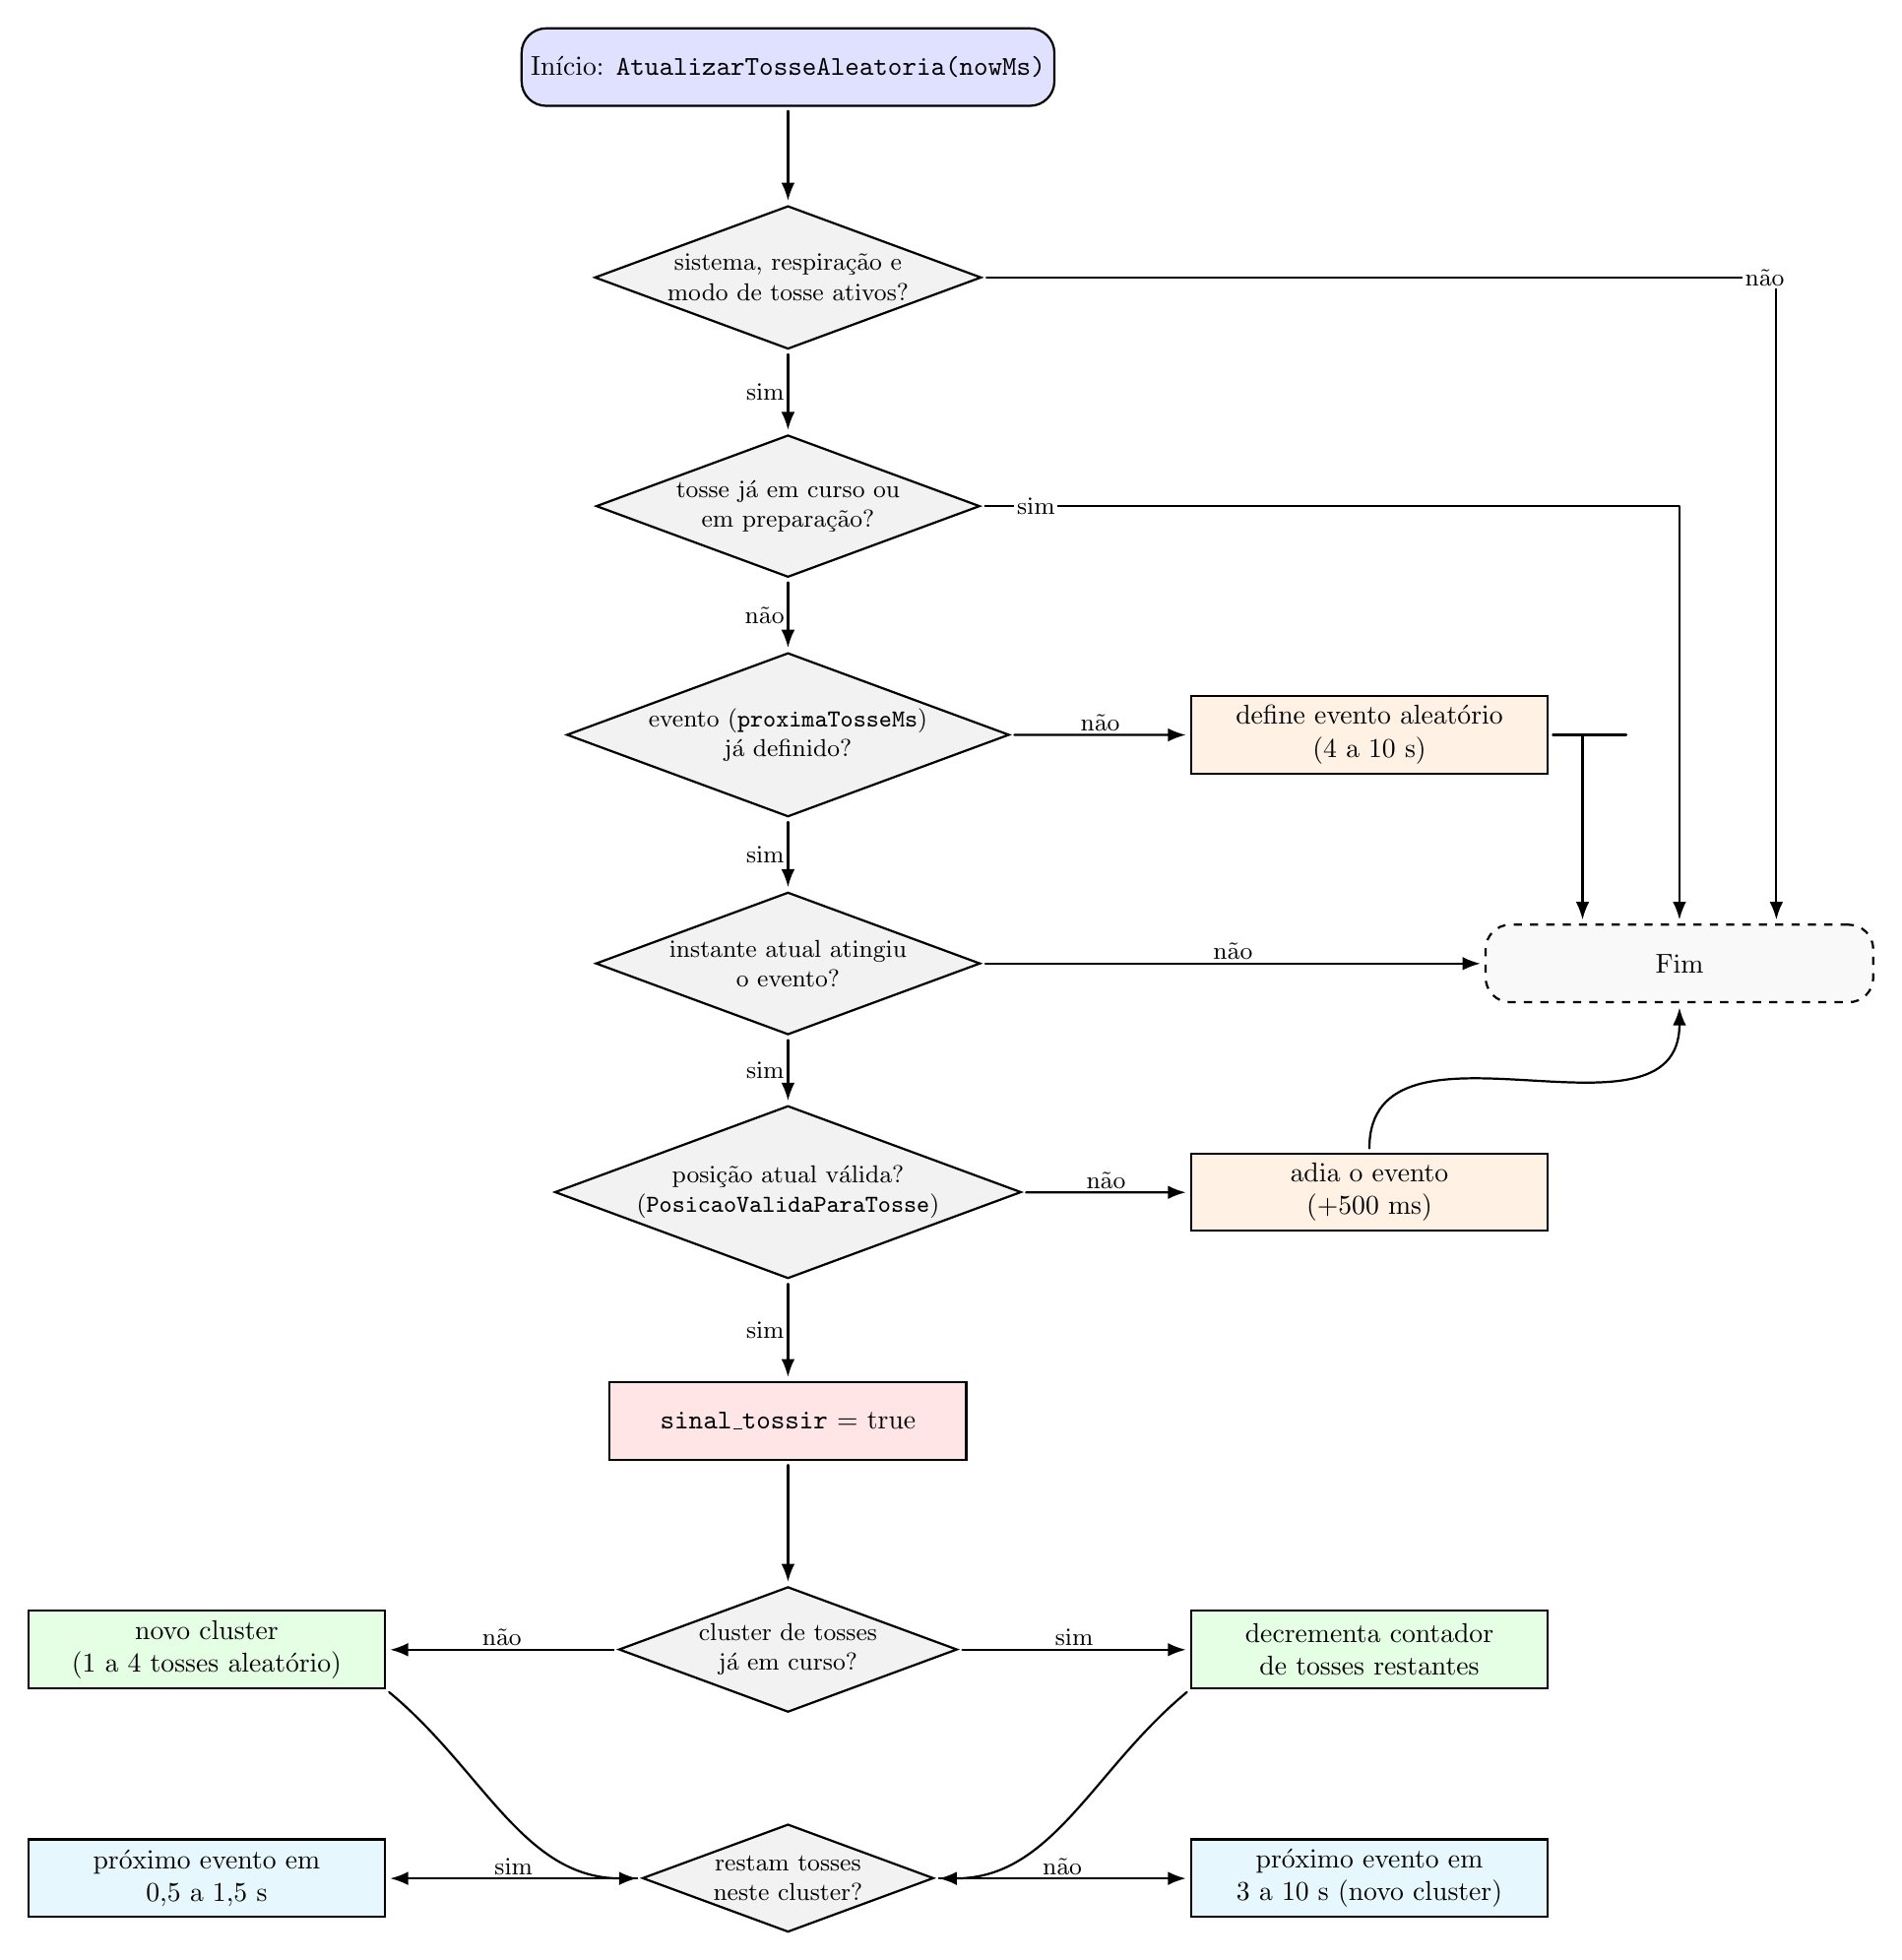
\begin{tikzpicture}[
    yscale=1.18,
    terminator/.style={draw, rounded corners=9pt, align=center, minimum width=5.0cm, minimum height=1.0cm, font=\normalsize, thick},
    process/.style={draw, align=center, minimum width=4.6cm, minimum height=1.0cm, font=\normalsize, thick},
    decision/.style={draw, diamond, aspect=2.7, align=center, font=\small, thick, inner sep=1pt},
    arrow/.style={-Latex, thick, line cap=round, line join=round, shorten >=1.5pt, shorten <=1.5pt},
    lab/.style={font=\small, fill=white, inner sep=1pt}
  ]
    \node[terminator, fill=blue!12] (n0) at (0,0)     {Início: \texttt{AtualizarTosseAleatoria(nowMs)}};
    \node[decision, fill=gray!10]   (n1) at (0,-2.3)  {sistema, respiração e\\modo de tosse ativos?};
    \node[decision, fill=gray!10]   (n2) at (0,-4.8)  {tosse já em curso ou\\em preparação?};
    \node[decision, fill=gray!10]   (n3) at (0,-7.3)  {evento (\texttt{proximaTosseMs})\\já definido?};
    \node[process, fill=orange!10]  (n3a) at (7.5,-7.3) {define evento aleatório\\(4 a 10 s)};
    \node[decision, fill=gray!10]   (n4) at (0,-9.8)  {instante atual atingiu\\o evento?};
    \node[decision, fill=gray!10]   (n5) at (0,-12.3) {posição atual válida?\\(\texttt{PosicaoValidaParaTosse})};
    \node[process, fill=orange!10]  (n5a) at (7.5,-12.3) {adia o evento\\(+500 ms)};
    \node[process, fill=red!10]     (n6) at (0,-14.8) {\texttt{sinal\_tossir} = true};
    \node[decision, fill=gray!10]   (n7) at (0,-17.3) {cluster de tosses\\já em curso?};
    \node[process, fill=green!10]   (n7a) at (-7.5,-17.3) {novo cluster\\(1 a 4 tosses aleatório)};
    \node[process, fill=green!10]   (n7b) at (7.5,-17.3)  {decrementa contador\\de tosses restantes};
    \node[decision, fill=gray!10]   (n8) at (0,-19.8) {restam tosses\\neste cluster?};
    \node[process, fill=cyan!10]    (n8a) at (-7.5,-19.8) {próximo evento em\\0,5 a 1,5 s};
    \node[process, fill=cyan!10]    (n8b) at (7.5,-19.8)  {próximo evento em\\3 a 10 s (novo cluster)};
    \node[terminator, dashed, fill=gray!5] (exit) at (11.5,-9.8) {Fim};
    \coordinate (exitTopLeft) at ($(exit.north)+(-1.25,0)$);
    \coordinate (exitTopMid) at ($(exit.north)+(0,0)$);
    \coordinate (exitTopRight) at ($(exit.north)+(1.25,0)$);

    \draw[arrow] (n0) -- (n1);
    \draw[arrow] (n1) -- node[lab, left]{sim} (n2);
    \draw[arrow] (n1.east) -- ++(4.3,0) -| (exitTopRight);
    \node[lab] at (12.6,-2.3) {não};
    \draw[arrow] (n2) -- node[lab, left]{não} (n3);
    \draw[arrow] (n2.east) -- ++(3.8,0) -| (exitTopMid);
    \node[lab] at (3.2,-4.8) {sim};
    \draw[arrow] (n3) -- node[lab, left]{sim} (n4);
    \draw[arrow] (n3) -- node[lab, above]{não} (n3a);
    \draw[arrow] (n3a.east) -- ++(1.0,0) -| (exitTopLeft);
    \draw[arrow] (n4) -- node[lab, left]{sim} (n5);
    \draw[arrow] (n4.east) -- node[lab, above]{não} (exit.west);
    \draw[arrow] (n5) -- node[lab, left]{sim} (n6);
    \draw[arrow] (n5) -- node[lab, above]{não} (n5a);
    \draw[arrow] (n5a.north) to[out=90, in=-90] (exit.south);
    \draw[arrow] (n6) -- (n7);
    \draw[arrow] (n7.west) -- node[lab, above]{não} (n7a.east);
    \draw[arrow] (n7.east) -- node[lab, above]{sim} (n7b.west);
    \draw[arrow] (n7a.south east) to[out=-35, in=180] (n8.west);
    \draw[arrow] (n7b.south west) to[out=-145, in=0] (n8.east);
    \draw[arrow] (n8.west) -- node[lab, above]{sim} (n8a.east);
    \draw[arrow] (n8.east) -- node[lab, above]{não} (n8b.west);
  \end{tikzpicture}}}
  \caption{Fluxograma da função \texttt{AtualizarTosseAleatoria()}.}
  \label{fig:tosse-aleatoria}
\end{figure}

\end{document}
